\themaE
\graphicspath{{../../S21_Le_parallelogramme/Images/}}

\chapter{Le parallélogramme}
\label{S21}


%%%%%%%%%%%%%%%%%%%%%%%%%%%%%%%
%%%%%%%%%%%%%%%%%%%%%%%%%%%%%%%
\begin{autoeval}
   \small
   \begin{enumerate}
      \item À partir des connaissances d'une définition et d'une propriété caractéristique du parallélogramme, il met en \oe uvre et écrit un protocole de construction.
      \item Il mène des raisonnements en utilisant des propriétés des figures, des configurations.
   \end{enumerate}
\end{autoeval}

\begin{prerequis}
   \begin{itemize}
      \item Parallélogramme (une définition et une propriété caractéristique).
      \item[\com] Mettre en oeuvre ou écrire un protocole de construction d’une figure géométrique.
   \end{itemize}
\end{prerequis}

\vfill

\begin{debat}[Défi : vocabulaire des quadrilatères]
   Le mot {\bf quadrilatère} provient du latin : {\it quatuor}, quatre, et {\it latus}, côté. Il existe un mot équivalent d'origine grecque : {\bf tétrapleure} de {\it tèssera}, quatre, et {\it pleura}, côté ou {\bf tétragone}, de {\it gônia}, angle. \\
   Comme pour les triangles, les quadrilatères peuvent être particuliers selon qu'ils ont certaines propriétés : parmi ceux-ci, on peut trouver par exemple la famille des trapèzes, des parallélogrammes, des rectangles, des losanges, des carrés ou encore des cerfs-volants. \\
   \begin{center}
      {\psset{unit=0.6}
      \begin{pspicture}(-1,-0.5)(14,7.5)
         \psframe[linecolor=red](7.25,0.25)(9.75,7.5)
         \psframe[linecolor=yellow](0.5,0.5)(9.5,2.5)
         \psframe[linecolor=orange](4.25,0)(10,5)
         \psframe[linecolor=orange!50](0.25,-0.25)(10.25,5.25)
         \psframe[linecolor=red!50](0,-0.5)(10.5,7.75)
         \psframe[linecolor=blue](-0.25,-0.75)(13.75,8)
         \psset{fillstyle=solid}
         \psframe[fillcolor=yellow](8,1)(9,2) %carré
         \psframe[fillcolor=yellow!50](5,1)(7,2) %rectangle
         \pspolygon[fillcolor=yellow!25](1,1)(3,1)(3,2)(1.5,2) %trapèze rectangle
         \pspolygon[fillcolor=orange!25](1,3.5)(3.5,3.5)(2.5,4.5)(1.5,4.5) %trapèze
         \pspolygon[fillcolor=orange!50](4.5,3.5)(6.25,3.5)(6.75,4.5)(5,4.5) %parallélogramme
         \pspolygon[fillcolor=orange](7.5,4)(8.5,3.5)(9.5,4)(8.5,4.5) %losange
         \pspolygon[fillcolor=red!50](3,6.5)(3,7)(5,7.5)(4.5,6) %convexe
         \pspolygon[fillcolor=red](8,6.75)(8.5,7.25)(9,6.75)(8.5,5.5) %cerf-volant
         \pspolygon[fillcolor=cyan!50](11,1.5)(13.5,3)(13,1.5)(11.25,2.5) %croisé
         \pspolygon[fillcolor=cyan](11,5)(13,5)(12.5,7)(12,5.5) %concave
      \end{pspicture}}
   \end{center}
   \bigskip
   \begin{cadre}[B2][J4]
      \begin{center}
         Vidéo : \href{https://www.yout-ube.com/watch?v=j_seCDgA-lU}{\bf Pourquoi \og mathématiques \fg{} ?}, site Internet {\it m@ths-et-tiques} de {\it Yvan Monka}.
      \end{center}
   \end{cadre}
\end{debat}


%%%%%%%%%%%%%%%%%%%%%%%%%%%%%%%%%%%%
%%%%%%%%%%%%%%%%%%%%%%%%%%%%%%%%%%%%
\activites

\begin{activite}[Les bandelettes]
   {\bf Objectifs :} connaître et reconnaître des figures à quatre côtés ; donner des propriétés de quadrilatères.
   \begin{QCM}
      \partie[construction des bandelettes]
         \begin{enumerate}
            \item On veut fabriquer à l'aide de bandelettes de papier des \og squelettes \fg{} de quadrilatères : chaque squelette est composé de deux bandelettes fixées à l'aide d'une attache parisienne. Sur une feuille de papier canson, tracer les deux rectangles suivants et placer les points O, O', M, N, P, Q, R et S à l'aide de la droite graduée en centimètres.
            \begin{center}
               \begin{pspicture}(-7,-2)(7,1.25)
                  \psline{->}(-6.5,-1.5)(6.5,-1.5)
                  \multido{\n=-6+1}{13}{\psline(\n,-1.6)(\n,-1.4)\rput(\n,-1.8){\footnotesize\n}}
                  \psline{<->}(-6.3,-1)(-6.3,1)
                  \rput{90}(-6.6,0){\footnotesize 2 cm}
                  \psframe[linewidth=0.5mm](-6,-1)(6,1)
                  \psline[linestyle=dashed,linecolor=gray](-6,0)(6,0)
                  \psdot[linewidth=2mm](0,0)
                  \rput(0,0.5){O}
                  \psdots[linewidth=0.5mm,linecolor=blue](-5,0)(-3,0)(3,0)(5,0)
                  \rput(-5,0.5){\blue M}
                  \rput(5,0.5){\blue N}
                  \psdots[linewidth=0.5mm,linecolor=red](-3,0)(3,0)
                  \rput(-3,0.5){\red P}
                  \rput(3,0.5){\red Q}     
               \end{pspicture} \\
               \begin{pspicture}(-7,-1.25)(7,1)
                  \psline{<->}(-6.3,-1)(-6.3,1)
                  \rput{90}(-6.6,0){\footnotesize 2 cm}
                  \psframe[linewidth=0.5mm](-6,-1)(6,1)
                  \psline[linestyle=dashed,linecolor=gray](-6,0)(6,0)t
                  \psdots[linewidth=2mm](0,0)
                  \rput(0,0.5){O'}
                  \psdots[linewidth=0.5mm,linecolor=teal](-5,0)(5,0)
                  \rput(-5,0.5){\textcolor{teal}{R}}
                  \rput(5,0.5){\textcolor{teal}{S}}   
               \end{pspicture}
            \end{center}
            \item Percer des trous sur les points M, N, P, Q, R et S qui doivent permettre de passer la mine d'un crayon. 
            \item Percer des trous sur les points O et O', qui sont destinés à recevoir une attache parisienne. \\
               Les bandelettes attachées correspondent alors au squelette d'un quadrilatère.
         \end{enumerate}

      \partie[construction des quadrilatères]
         \begin{enumerate}
         \setcounter{enumi}{3}
            \item On considère un squelette obtenu en faisant se croiser les deux bandelettes aux points O et O' en plaçant l'attache parisienne à travers ces deux points. On s'intéresse aux quadrilatères MRNS tracés à partir de ce squelette.
            \begin{enumerate}
               \item En plaçant le squelette sur votre feuille, placer les points M, N, R et S puis tracer le quadrilatère MRNS.
               \item À quelle famille semble appartenir ce quadrilatère ?
               \item Que représentent les segments [MN] et [RS] pour ce quadrilatère ?
               \item Justifier alors la conjecture proposée en b).
               \item Citer d'autres propriétés relatives à ce quadrilatère particulier.
               \item Trouver un cas particulier à cette configuration.
            \end{enumerate}
            \item On s'intéresse maintenant aux quadrilatères PRQS tracés à partir de ce même squelette.
            \begin{enumerate}
               \item En plaçant le squelette sur votre feuille, placer les points P, Q, R et S puis tracer le quadrilatère PRQS.
               \item À quelle famille semble appartenir ce quadrilatère ?
               \item Que représentent les segments [PQ] et [RS] pour ce quadrilatère ?
               \item Conjecturer trois propriétés concernant votre quadrilatère : une à partir de ses diagonales, une autre à partir de la position relative de ses côtés et une dernière concernant les angles.
                \item Trouver un cas particulier à cette configuration.
            \end{enumerate}
      \end{enumerate}
\end{QCM}
  
     \vfill\hfill{\it\footnotesize Source : inspirée du site de \href{http://pernoux.pagesperso-orange.fr/revision/revgeo.pdf}{Dominique Pernoux}}.
\end{activite}


%%%%%%%%%%%%%%%%%%%%%%%%%%%%%
%%%%%%%%%%%%%%%%%%%%%%%%%%%%%
\cours 

\begin{definition}
   Un {\bf parallélogramme} est un quadrilatère dont les côtés sont deux à deux parallèles.
\end{definition}

\begin{center}
   \small
   {\psset{yunit=0.5}
   \begin{pspicture}(0,0.2)(8,4.3)
     \psline[linecolor=A1](0.5,0)(2.5,4)
      \psline[linecolor=A1](3.5,0.5)(5.5,4.5)
      \psline[linecolor=B1](0,1)(5,1.5)
      \psline[linecolor=B1](1,3)(6,3.5)
      \rput[rt](0.8,0.95){$A$}
      \rput[lt](4,1.15){$B$}
      \rput[lb](5.25,3.6){$C$}
      \rput[rb](2.1,3.3){$D$}
      \rput(7,2){$\Longrightarrow$}
      \rput(7,2.7){$(AB)//(DC)$}
      \rput(7,1.3){$(AD)//(BC)$}
   \end{pspicture}
   \begin{pspicture}(0,0.2)(6,4.3)
      \pstGeonode[CurveType=polygon,PointSymbol=none,PosAngle={-135,-45,45,135}](1,1){A}(4,1.5){B}(5,3.5){C}(2,3){D}
      \rput(3,2.25){parallélogramme}
   \end{pspicture}}
\end{center}
  
Autres caractéristiques d'un parallélogramme :

\begin{tableau}[pr]{\linewidth}
   \hline %%%%%%%%%%%%%%%%%%%%%%%%%%
   \begin{pspicture}(-0.25,0)(3,1.75)
       \footnotesize
       \psset{linewidth=0.2mm}
       \pstGeonode[PointSymbol=none,CurveType=polygon,PosAngle={-135,-45,45,135}]{A}(2.5,0.5){B}(3,1.5){C}(0.5,1){D}
       \pstGeonode[PointName=none,PointSymbol=none](1.5,0.75){O}
       \pstLineAB{A}{C}
       \pstLineAB{B}{D}
       \pstSegmentMark[SegmentSymbol=MarkCros,linecolor=A1]{O}{A}
       \pstSegmentMark[SegmentSymbol=MarkCros,linecolor=A1]{O}{C}
       \pstSegmentMark[linecolor=B1]{O}{B}
       \pstSegmentMark[linecolor=B1]{O}{D}
   \end{pspicture}
   &
   \propriete{} Si un quadrilatère a ses diagonales qui se coupent en leur milieu alors c'est un parallélogramme.
   &
   Ici, $[AC]$ et $[BD]$ se coupent en leur milieu, donc, $ABCD$ est un parallélogramme. \\
   \hline %%%%%%%%%%%%%%%%%%%%%%%%%
   \begin{pspicture}(-0.25,0)(3,1.75)
       \footnotesize
       \psset{linewidth=0.2mm}
       \pstGeonode[PointSymbol=none,CurveType=polygon,PosAngle={-135,-45,45,135}]{A}(2.5,0.5){B}(3,1.5){C}(0.5,1){D}
       \pstGeonode[PointName=none,PointSymbol=none](1.5,0.75){O}
       \pstSegmentMark[SegmentSymbol=MarkCross,linecolor=A1]{A}{B}
       \pstSegmentMark[SegmentSymbol=MarkCross,linecolor=A1]{D}{C}
       \pstSegmentMark[SegmentSymbol=MarkHash,linecolor=B1]{C}{B}
       \pstSegmentMark[SegmentSymbol=MarkHash,linecolor=B1]{A}{D}
   \end{pspicture}
   &
   \propriete{} Si un quadrilatère a ses côtés opposés de la même longueur deux à deux alors c'est un parallélogramme.
   &
   Ici, $AB=DC$ et $AD=BC$, donc, $ABCD$ est un parallélogramme. \\
   \hline
   \begin{pspicture}(-0.25,0)(3,1.75)
       \footnotesize
       \psset{linewidth=0.2mm}
       \pstGeonode[PointSymbol=none,CurveType=polygon,PosAngle={-135,-45,45,135}]{A}(2.5,0.5){B}(3,1.5){C}(0.5,1){D}
       \pstGeonode[PosAngle=90](1.5,0.75){O}
       \pstMarkAngle[linecolor=A1]{B}{A}{D}{}
       \pstMarkAngle[linecolor=A1]{D}{C}{B}{}
       \pstMarkAngle[linecolor=B1,MarkAngleRadius=0.2]{A}{D}{C}{}
       \pstMarkAngle[linecolor=B1,MarkAngleRadius=0.3]{A}{D}{C}{}
       \pstMarkAngle[linecolor=B1,MarkAngleRadius=0.2]{C}{B}{A}{}
       \pstMarkAngle[linecolor=B1,MarkAngleRadius=0.3]{C}{B}{A}{}
   \end{pspicture}
   &
   \propriete{} Un parallélogramme possède son centre $O$ comme centre de symétrie. \newline
   Les angles opposés sont égaux.
   &
   Ici, $\widehat{ADC} =\widehat{ABC}$ et $\widehat{DAB} =\widehat{DCB}$. \\
   \hline
\end{tableau}

\vspace*{-5mm}

\section{Parallélogrammes particuliers} %%%

\begin{center}
   {\small
   \psset{unit=0.9}
   \begin{pspicture}(0,1)(16,8)
      \pspolygon(0,3)(3,3)(4,5)(1,5) 
      \psframe(7,5.5)(10,7.5)
      \pspolygon(6.5,1.5)(8.5,0.5)(10.5,1.5)(8.5,2.5)
      \psframe(13.5,2.75)(16,5.25)
      \psline[linestyle=dashed]{->}(3,5.5)(6.5,6.5)
      \rput{18}(4.6,6.3){+ angle $\square$}
      \rput{18}(4.9,5.65){+ diag. =}
      \psline[linestyle=dashed]{->}(3,2.5)(6,1.5)
      \rput{-18}(4.35,1.65){+ long. =}
      \rput{-18}(4.7,2.3){+ diag. $\perp$}
      \psline[linestyle=dashed]{->}(10.5,6.5)(13,5.5)
      \rput{30}(12.2,1.7){+ angle $\square$}
      \rput{30}(11.8,2.25){+ diag. =}
      \psline[linestyle=dashed]{->}(11,1.5)(13,2.5)
      \rput{-20}(11.9,6.3){+ long. =}
      \rput{-20}(11.6,5.7){+ diag. $\perp$}
      \psset{linecolor=B1}
         \psline(0,3)(4,5)
         \psline(1,5)(3,3)
         \psline(7,5.5)(10,7.5)
         \psline(7,7.5)(10,5.5)
         \psline(6.5,1.5)(10.5,1.5)
         \psline(8.5,0.5)(8.5,2.5)
         \psline(13.5,5.25)(16,2.75)
         \psline(13.5,2.75)(16,5.25)
      \textcolor{A1}{
         \rput(1.5,3){x}
         \rput(2.5,5){x}
         \rput(0.5,4){$\approx$}
         \rput(3.5,4){$\approx$}
         \rput(1.5,4.5){$\circ$}
         \rput(2.5,3.5){$\circ$}
         \rput{30}(1,3.5){|}
         \rput{30}(3,4.5){|}
         \rput(8.5,5.5){x}
         \rput(8.5,7.5){x}
         \rput(7,6.5){$\approx$}
         \rput(10,6.5){$\approx$}
         \rput(7.75,6){$\circ$}
         \rput(7.75,7){$\circ$}
         \rput(9.25,6){$\circ$}
         \rput(9.25,7){$\circ$}
         \rput(13.5,4){x}
         \rput(16,4){x}
         \rput(14.75,2.75){x}
         \rput(14.75,5.25){x}
         \rput(14.125,3.375){$\circ$}
         \rput(15.375,4.625){$\circ$}
         \rput(14.125,4.625){$\circ$}
         \rput(15.375,3.375){$\circ$}
         \rput(7.5,1){x}
         \rput(7.5,2){x}
         \rput(9.5,1){x}
         \rput(9.5,2){x}
         \rput(7.5,1.5){$\circ$}
         \rput(9.5,1.5){$\circ$}
         \rput{90}(8.5,1){|}
         \rput{90}(8.5,2){|}
         \psset{linecolor=blue}
         \psframe(7,5.5)(7.3,5.8)
         \psframe(8.5,1.5)(8.8,1.8)
         \psframe(13.5,2.75)(13.8,3.05)
         \pspolygon(14.75,4)(14.95,4.2)(14.75,4.4)(14.55,4.2)}
   \end{pspicture}}
\end{center}


%%%%%%%%%%%%%%%%%%%%%%%%%%%%%%%%%%%%%%%%
%%%%%%%%%%%%%%%%%%%%%%%%%%%%%%%%%%%%%%%%
\exercicesbase

\begin{colonne*exercice}

\begin{exercice} %1
   On considère le parallélogramme $ILAN$ suivant :
   \begin{center}
      \begin{pspicture}(-0.5,-0.25)(5,2.5)
         \footnotesize
         \pstGeonode[PointSymbol=none,CurveType=polygon,PosAngle={-135,-45,45,135}]{I}(3.5,0){L}(4.5,2){A}(1,2){N}
         \pstGeonode[PosAngle=90,PointSymbol=none](2.25,1){O}
         \pstLineAB{L}{N}
         \pstLineAB{I}{A}
      \end{pspicture}      
   \end{center}
   Coder un maximum d'informations sur la figure.
\end{exercice}
      
\begin{corrige}
   \ \\
   \begin{pspicture}(-1,-0.5)(5,2)
      {\footnotesize
      \pstGeonode[PointSymbol=none,CurveType=polygon,PosAngle={-135,-45,45,135}]{I}(3.5,0){L}(4.5,2){A}(1,2){N}
      \pstGeonode[PosAngle=90,PointSymbol=none](2.25,1){O}
      \pstLineAB{L}{N}
      \pstLineAB{I}{A}    
      \pstSegmentMark{I}{L}
      \pstSegmentMark{N}{A}
      \pstSegmentMark[SegmentSymbol=MarkHash]{N}{I}
      \pstSegmentMark[SegmentSymbol=MarkHash]{L}{A}
      \pstSegmentMark[SegmentSymbol=MarkCros]{O}{I}
      \pstSegmentMark[SegmentSymbol=MarkCros]{O}{A}
      \pstSegmentMark[SegmentSymbol=MarkArrow]{O}{N}
      \pstSegmentMark[SegmentSymbol=MarkArrow]{L}{O}
      \psset{linecolor=blue}
      \pstMarkAngle{L}{I}{N}{}
      \pstMarkAngle{N}{A}{L}{}
      \pstMarkAngle[MarkAngleRadius=0.2]{I}{N}{A}{}
      \pstMarkAngle[MarkAngleRadius=0.3]{I}{N}{A}{}
      \pstMarkAngle[MarkAngleRadius=0.2]{A}{L}{I}{}
      \pstMarkAngle[MarkAngleRadius=0.3]{A}{L}{I}{}}
   \end{pspicture}
\end{corrige}

\bigskip


\begin{exercice} %2
   Dans les parallélogrammes $ROSE$ et $BLEU$ suivants, compléter toutes les mesures possibles.
   \begin{center}
   {\psset{unit=0.8}
      \begin{pspicture}(5,2.5)
         \footnotesize
         \pspolygon(0,0)(3.5,0)(4.5,2)(1,2) 
         \psline(0,0)(4.5,2)
         \psline(3.5,0)(1,2)
         \rput(-0.2,0){$R$}
         \rput(3.8,0){$O$}
         \rput(4.8,2){$S$}
         \rput(0.7,2){$E$}
         \rput{-38}(3,0.7){\ucm{3}}
         \rput{29}(1.2,0.8){\ucm{4}}
      \end{pspicture}
      \begin{pspicture}(3,2.5)
         \footnotesize
         \pspolygon(0,0)(2.5,0)(3.5,2)(1,2) 
         \rput(-0.25,0){$B$}
         \rput(2.8,0){$L$}
         \rput(3.75,2){$E$}
         \rput(0.7,2){$U$}
         \rput(1.4,0.25){\ucm{6}}
         \rput{62}(0.2,1){\ucm{4}}
         \psarc(3.5,2){0.5}{180}{-117}
         \rput(2.7,1.6){63\degre}
         \psarc(1,2){0.5}{-117}{0}
         \rput(1.5,1.4){117\degre}
      \end{pspicture}}
   \end{center}
\end{exercice}  

\begin{corrige}
   \ \\ [-5mm]
   {\psset{unit=0.8}
   \footnotesize
   \begin{pspicture}(5,2.3)
      \pspolygon(0,0)(3.5,0)(4.5,2)(1,2) 
      \psline(0,0)(4.5,2)
      \psline(3.5,0)(1,2)
      \rput(-0.2,0){$R$}
      \rput(3.8,0){$O$}
      \rput(4.8,2){$S$}
      \rput(0.7,2){$E$}
      \rput{-38}(3,0.7){\ucm{3}}
      \rput{24}(1.2,0.8){\ucm{4}}
      \rput{-38}(1.9,1.6){\blue \ucm{3}}
      \rput{24}(3,1.6){\blue \ucm{4}}
   \end{pspicture}
   \begin{pspicture}(3,2.3)
      \pspolygon(0,0)(2.5,0)(3.5,2)(1,2) 
      \rput(-0.25,0){$B$}
      \rput(2.8,0){$L$}
      \rput(3.75,2){$E$}
      \rput(0.7,2){$U$}
      \rput(1.4,0.25){\ucm{6}}
      \rput{62}(0.2,1){\ucm{4}}
      \rput(2.4,2.25){\blue \ucm{6}}
      \rput{62}(3.2,1){\blue \ucm{4}}
      \psarc(3.5,2){0.5}{180}{-117}
      \rput(2.7,1.6){\udeg{63}}
      \psarc[linecolor=blue](2.5,0){0.5}{63}{180}
      \rput(2.2,0.7){\blue \udeg{117}}
      \psarc[linecolor=blue](0,0){0.5}{0}{63}
      \rput(0.7,0.4){\blue \udeg{63}}
      \psarc(1,2){0.5}{-117}{0}
      \rput(1.5,1.4){\udeg{117}}
   \end{pspicture}}
\end{corrige} 

\bigskip


\begin{exercice} %3
   Construire sur ce quadrillage les parallélogrammes suivants : $ABCF$, $BCDG$, $CDHE$ et $BIEC$.
   \begin{center}
      {\psset{unit=0.7}
      \begin{pspicture}(11,11)
         \psgrid[subgriddiv=0,gridcolor=lightgray,gridlabels=0](0,0)(11,11)
         \pstGeonode(1,1){A}(5,1){B}(6,3){C}(9,6){D}(3,7){E}         
      \end{pspicture}}
   \end{center} 
\end{exercice}

\begin{corrige}
   \ \\ [-3mm]
   {\psset{unit=0.7}
      \begin{pspicture}(11,11)
         \psgrid[subgriddiv=0,gridcolor=lightgray,gridlabels=0](0,0)(11,11)
         \pstGeonode(1,1){A}(5,1){B}(6,3){C}(9,6){D}(3,7){E}
         \pstGeonode[CurveType=polygon,linecolor=A1](1,1){A}(5,1){B}(6,3){C}(2,3){F}
         \pstGeonode[CurveType=polygon,linecolor=B1](5,1){B}(6,3){C}(9,6){D}(8,4){G}
         \pstGeonode[CurveType=polygon,linecolor=G1](6,3){C}(9,6){D}(6,10){H}(3,7){E}
         \pstGeonode[CurveType=polygon,linecolor=J1](5,1){B}(2,5){I}(3,7){E}(6,3){C}
      \end{pspicture}}
\end{corrige}

\bigskip


\begin{exercice} %4
   Construire les parallélogrammes $ABCD$ et $EFGH$ tels que :
   \begin{enumerate}
      \item $AB =\ucm{5} \; ; AD =\ucm{3,5}$ et $BD =\ucm{7}$.
      \item $EF =\ucm{2} \; ; EH =\ucm{4,5}$ et $EG = \ucm{3,5}$.
   \end{enumerate}
\end{exercice}

\begin{corrige}
\ \\ [-5mm]
   \begin{enumerate}
      \item
      {\footnotesize
         \begin{pspicture}(-1.5,1.5)(6,3.8)
      \pstGeonode[PointSymbol=none,CurveType=polygon,PosAngle={-135,-45,45,135}]{A}(5,0){B}(3.8,3.3){C}(-1.2,3.3){D}
            \pstLineAB{D}{B}
            \pstLabelAB{D}{B}{\blue \ucm{7}}
            \pstLabelAB[offset=-3mm]{D}{A}{\blue \ucm{3,5}}
            \pstLabelAB[offset=-3mm]{A}{B}{\blue \ucm{5}}
            \pstSegmentMark[SegmentSymbol=MarkHash]{A}{D}
            \pstSegmentMark[SegmentSymbol=MarkHash]{B}{C}
            \pstSegmentMark[SegmentSymbol=MarkCros]{A}{B}
            \pstSegmentMark[SegmentSymbol=MarkCros]{D}{C}
         \end{pspicture}}
      \item
      {\footnotesize
         \begin{pspicture}(-2,0.5)(5,4.3)
      \pstGeonode[PointSymbol=none,CurveType=polygon,PosAngle={-135,-45,45,135}]{E}(4.5,0){H}(3.5;25.2){G}(2;131.8){F}
            \pstLineAB{E}{G}
            \pstLabelAB{E}{G}{\blue \ucm{3,5}}
            \pstLabelAB[offset=-4mm]{E}{H}{\blue \ucm{4,5}}
            \pstLabelAB[offset=-4mm]{F}{E}{\blue \ucm{2}}
            \pstSegmentMark[SegmentSymbol=MarkCros]{E}{F}
            \pstSegmentMark[SegmentSymbol=MarkCros]{H}{G}
            \pstSegmentMark[SegmentSymbol=MarkHashh]{E}{H}
           \pstSegmentMark[SegmentSymbol=MarkHashh]{F}{G}
      \end{pspicture}}
   \end{enumerate}
\end{corrige}

\bigskip


\begin{exercice} %5
   Construire en vraie grandeur les parallélogrammes schématisés ci-dessous (les longueurs sont en cm).
   \begin{center}
      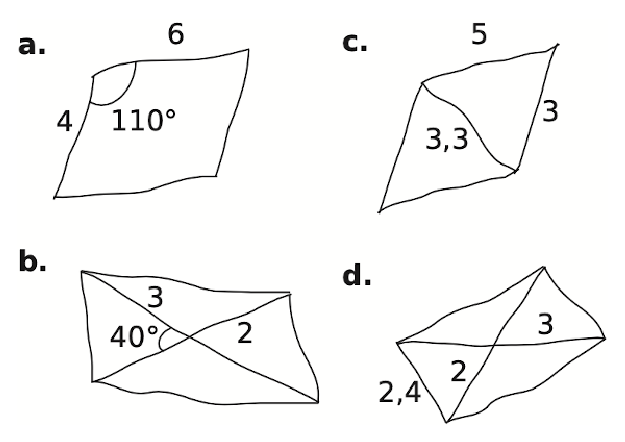
\includegraphics[width=8cm]{Parallelogramme_exo}
   \end{center}
\end{exercice}

\begin{corrige}
   \ \\ [-5mm] 
   \begin{pspicture}(0,-0.5)(7.5,4.5)
      \pstGeonode[PointSymbol=none,CurveType=polygon,PointName=none]{A}(6,0){B}(7.37,3.76){C}(4;70){D}
      \pstLabelAB{D}{C}{\blue \ucm{6}}
      \pstLabelAB{A}{D}{\blue \ucm{4}}
      \pstMarkAngle{A}{D}{C}{\blue \udeg{110}}
      \rput(0,3.7){\textcolor{G1}{\bf a.}}
   \end{pspicture} \\
   \begin{pspicture}(-3.5,-2)(3,2)
      \pstGeonode[PointSymbol=none,CurveType=polygon,PointName=none](3;180){A}(2;220){B}(3;0){C}(2;40){D}
      \pstGeonode[PointSymbol=none,PointName=none]{O}
      \pstLineAB{A}{C}
      \pstLineAB{B}{D}
      \pstLabelAB[offset=-2mm]{O}{D}{\blue\small \ucm{2}}
      \pstLabelAB[offset=2mm]{A}{O}{\blue\small \ucm{3}}
      \pstMarkAngle{A}{O}{B}{\blue \udeg{40}}
      \rput(-3,1){\textcolor{G1}{\bf b.}}
   \end{pspicture} \\
   \begin{pspicture}(0,-0.5)(3,2.5)
      \pstGeonode[PointSymbol=none,CurveType=polygon,PointName=none]{A}(5,0){B}(7.3,1.9){C}(3;39.6){D}
      \pstLineAB{B}{D}
      \pstLabelAB[offset=-3mm]{B}{C}{\blue\ucm{3}}
      \pstLabelAB{D}{C}{\blue\ucm{5}}
      \pstLabelAB[offset=-3mm]{D}{B}{\blue\ucm{3,3}}
      \rput(-0.1,1.8){\textcolor{G1}{\bf c.}}
   \end{pspicture} \\
   \begin{pspicture}(-3.5,-2)(3,2.5)
      \pstGeonode[PointSymbol=none,CurveType=polygon,PointName=none](3;180){A}(2;232.0){B}(3;0){C}(2;52.9){D}
      \pstGeonode[PointSymbol=none,PointName=none]{O}
      \pstLineAB{A}{C}
      \pstLineAB{B}{D}
      \pstLabelAB[offset=-3mm]{A}{B}{\blue\ucm{2,4}}
      \pstLabelAB{B}{O}{\blue\ucm{2}}
      \pstLabelAB{O}{C}{\blue\ucm{3}}
      \rput(-3.1,1.3){\textcolor{G1}{\bf d.}}
   \end{pspicture}
\end{corrige}

\smallskip


\begin{exercice} %6
   Construire en vraie grandeur :
   \begin{enumerate}
      \item Un parallélogramme $VERT$ tel que \\
         $VT = \ucm{5} \; ; \widehat{ERT} =\udeg{125}$ et $VE =\ucm{4}$.
      \item Un parallélogramme $GRIS$ de centre $O$ tel que \\
         $GR =\ucm{6} \; ; SO =\ucm{3}$ et $IO =\ucm{4}$.
      \item Un parallélogramme $NOIR$ tel que \\
         $NI =\umm{62} \; ; \widehat{NIR} =\udeg{40}$ et $\widehat{RNI} =\udeg{30}$.
   \end{enumerate}
\end{exercice}

\begin{corrige}
\ \\ [-5mm]
   \begin{enumerate}
      \item \\
      \begin{pspicture}(-2.3,0)(6,3.9)
      \pstGeonode[PointSymbol=none,CurveType=polygon,PosAngle={-135,135,45,-45}]{V}(4;125){E}(2.7,3.3){R}(5,0){T}
         \pstLabelAB[offset=-3mm]{V}{T}{\blue\ucm{5}}
         \pstLabelAB[offset=-3mm]{E}{V}{\blue\ucm{4}}
        \pstMarkAngle{E}{R}{T}{\blue\udeg{125}}
      \end{pspicture}
   \end{enumerate}
   
\Coupe

   \begin{enumerate}
   \setcounter{enumi}{1}
      \item \\
      \begin{pspicture}(0,-0.5)(7,3.4)         \pstGeonode[PointSymbol=none,CurveType=polygon,PosAngle={-135,-45,45,135}]{G}(6,0){R}(8;26.4){I}(1.2,3.6){S}
         \pstGeonode[PointSymbol=none,PosAngle=90](4;26.4){O}
         \pstLineAB{G}{I}
         \pstLineAB{R}{S}
         \pstLabelAB[offset=-3mm]{G}{R}{\blue\ucm{6}}
         \pstLabelAB{S}{O}{\blue\ucm{3}}
         \pstLabelAB{O}{I}{\blue\ucm{4}}
      \end{pspicture}
      \item \\
      \begin{pspicture}(0,-2.2)(6,2.2)
         \pstGeonode[PointSymbol=none,CurveType=polygon,PosAngle={180,-90,0,90}]{N}(3.35;-40){O}(6.3,0){I}(4.3;30){R}
         \pstLineAB{N}{I}
         \pstLabelAB{N}{I}{\blue\umm{62}}
         \pstMarkAngle{R}{I}{N}{\blue\udeg{40}}
         \pstMarkAngle{I}{N}{R}{\blue\udeg{30}}
      \end{pspicture}
   \end{enumerate}
\end{corrige}

\bigskip


\begin{exercice} %7
   Tracer, puis démontrer\dots
   \begin{enumerate}
      \item Tracer le cercle $(C_1)$ de centre $O$ de rayon \ucm{3,5}.
      \item Placer deux points $N$ et $P$ sur $(C_1)$ tels que [NP] soit un diamètre de $(C_1)$.
      \item Construire le cercle $(C_2)$ de centre $O$ de rayon \ucm{5}.
      \item Placer deux autres points $Q$ et $R$ sur $(C_2)$, non alignés avec $N$ et $P$ tels que $[QR]$ soit un diamètre de $(C_2)$.
      \item Démontrer que le quadrilatère $NQPR$ est un parallélogramme.
      \item Calculer les longueurs $NP$ et $QR$. Justifier.
   \end{enumerate} 
\end{exercice}

\begin{corrige}
   Questions 1 à 4. Figure à l'échelle trois quarts : \\
   {\psset{unit=0.75}
   \begin{pspicture}(-4.5,-5)(5,5.3)
      \pscircle(0,0){3.5}
      \pscircle(0,0){5}
      \psline(3.5;240)(3.5;60)
      \psline(5;190)(5;10)
      \pspolygon[linecolor=blue](3.5;240)(5;190)(3.5;60)(5;10)
      \rput(3.8;240){N}
      \rput(5.3;190){Q}
      \rput(3.8;60){P}
      \rput(5.3;10){R}
      \rput(3.9;110){$(C_1)$}
      \rput(5.5;150){$(C_2)$}
      \rput{60}(0.5,1.5){\blue\ucm{3,5}}
      \rput{12}(2,0.7){\blue\ucm{5}}
      \rput(-0.2,0.4){$O$}
   \end{pspicture}}
   \begin{enumerate}
   \setcounter{enumi}{4}
      \item $O$ est le milieu du segment $[QR]$ et également le milieu du segment $[NP]$. Or, ces deux segments sont les diagonales du quadrilatère $NQPR$ donc, ses diagonales se coupent en leur milieu et par conséquent : {\blue $NQPR$ est un parallélogramme}.
      \item $NP =2OP =2\times\ucm{3,5} =\blue\ucm{7}$. \\
         $QR =2OR =2\times\ucm{5} =\blue\ucm{10}$.
   \end{enumerate}
\end{corrige}

\bigskip


\begin{exercice} %8
   Tracer, puis démontrer\dots{} le retour !
   \begin{enumerate}
      \item Tracer un triangle équilatéral $ABC$ de côté \ucm{5}.
      \item À l'extérieur du triangle et de telle sorte que les figures ne se recouvrent pas, placer les points $D$ et $E$ tels que $ABDE$ soit un rectangle avec $AD =\ucm{7}$.
      \item Placer les points $F$ et $G$ tels que $ACFG$ soit un losange avec $\widehat{ACF} =\udeg{150}$.
      \item Donner la mesure des angles $\widehat{CAG}$ et $\widehat{BAG}$.
      \item Que peut-on en déduire pour les points $G, A$ et $E$ ?
   \end{enumerate}
\end{exercice}

\begin{corrige}
   \ \\ [-5mm]
   \begin{enumerate}
      \item {\bf\textcolor{G1}{2) \;3)}} Figure taille réelle.
      \begin{pspicture}(-1,-5.7)(5,10.2)
         \pstGeonode[PointSymbol=none,PosAngle={180,0,45,-45,-135,45,145}]{A}(5,0){B}(5;60){C}(5,-5){D}(0,-5){E}(2.8,9.5){F}(0,5){G}
         \psset{MarkAngle=90}
         \pstSegmentMark{A}{B}
         \pstSegmentMark{B}{C}
         \pstSegmentMark{A}{C}
         \pstLabelAB{A}{B}{\blue\ucm{5}}
         \pstSegmentMark[SegmentSymbol=pstslashhh]{B}{D}
         \pstSegmentMark[SegmentSymbol=pstslashhh]{A}{E}
         \pstSegmentMark{E}{D}
         \pstLabelAB{A}{D}{\blue\ucm{7}}
         \pstSegmentMark{C}{F}
         \pstSegmentMark{F}{G}
         \pstSegmentMark{A}{G}
         \pstLineAB{A}{D}
         \pstMarkAngle[Mark=MarkHashhh,MarkAngleRadius=0.5]{F}{C}{A}{\blue\udeg{150}}
         \pstMarkAngle{B}{A}{C}{\blue\udeg{60}}
         \pstMarkAngle{C}{B}{A}{\blue\udeg{60}}
         \pstMarkAngle{A}{C}{B}{\blue\udeg{60}}
         \pstRightAngle{A}{B}{D}
      \end{pspicture}
      \setcounter{enumi}{3}
      \item Le triangle $CAG$ est isocèle en $A$ puisque $AC = AG$ donc, $\widehat{ACG} = \widehat{AGC}$. \\
      De plus, $(GC)$ est un axe de symétrie du losange, donc $\widehat{ACG}=\udeg{150}\div2 =\udeg{75}$. \\
      La somme des angles dans un triangle vaut \udeg{180} donc $\widehat{CAG}+\widehat{AGC}+\widehat{GCA} =\udeg{180}$ soit $\widehat{CAG} + \udeg{75}+\udeg{75}=\udeg{180}$ ou encore {\blue $\widehat{CAG} =\udeg{30}$}. \\
      $\widehat{BAG} = \widehat{BAC}+\widehat{CAG} =\udeg{60}+\udeg{30} =\blue \udeg{90}$. \smallskip
      \item On a $\widehat{GAE} =\widehat{GAB}+\widehat{BAE} =\udeg{90}+\udeg{90} =\udeg{180}$ donc l'angle $\widehat{GAE}$ est plat d'où : {\blue les points $G, A$ et $E$ sont alignés}.
   \end{enumerate}
\end{corrige}

\end{colonne*exercice}


%%%%%%%%%%%%%%%%%%%%%%%%%%%%%%%%%%%
%%%%%%%%%%%%%%%%%%%%%%%%%%%%%%%%%%%
\Recreation

\begin{enigme}[Les puzzles de Sam Loyd]

   Sam Loyd (1841-1911) était un mathématicien américain adepte de casse-têtes mathématiques et d'échec. Il est à l'origine de milliers de casse-têtes publiés notamment dans des journaux. On considère l'énigme \og The royal road to mathematics \fg{}, issu du {\it Sam Loyd's cyclopedia of 5000 puzzles tricks and conundrums with answers}, page 60.
   \begin{center}
      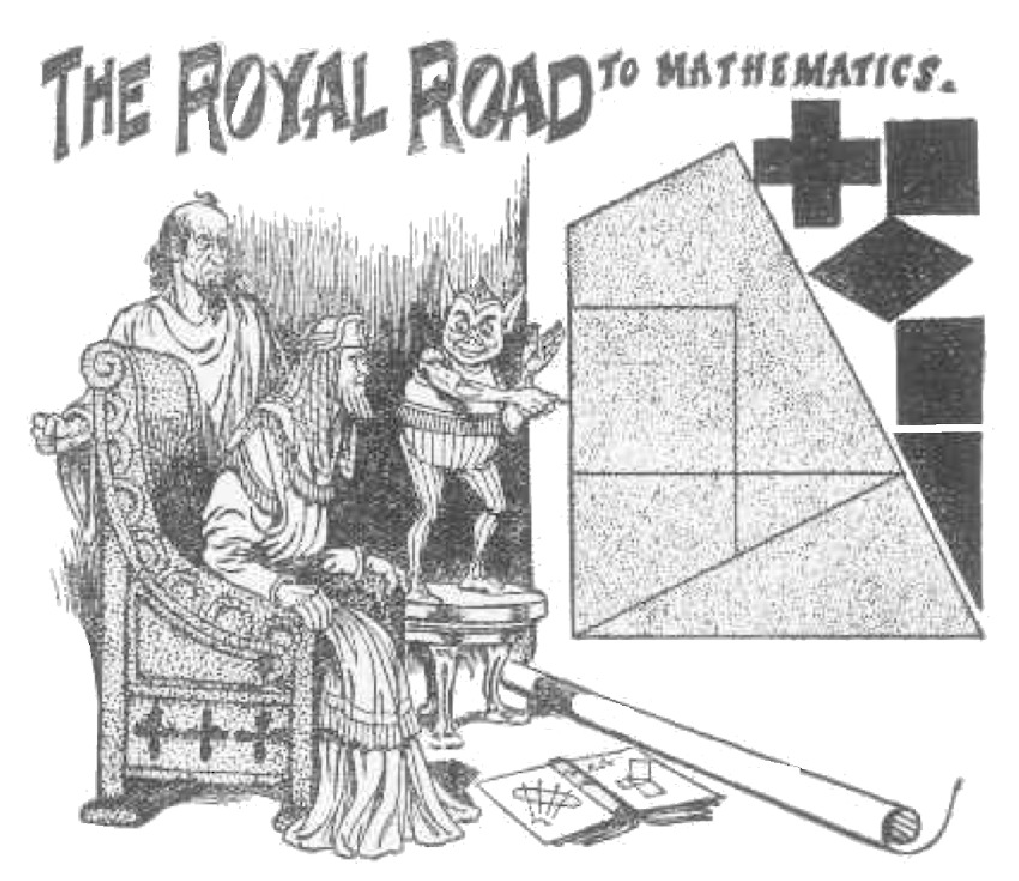
\includegraphics[width=9cm]{Sam_loyd} \quad 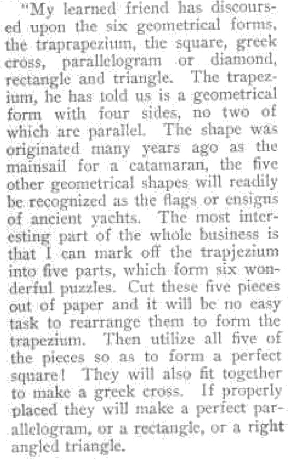
\includegraphics[width=5cm]{Sam_loyd_texte}
   \end{center}
   \begin{multicols}{2}
      \partie[composition du trapezium]
      On considère le quadrilatère de Sam Loyd \\
      construit sur le quadrillage suivant : \\
         {\psset{unit=0.9}
         \begin{pspicture}(-1.5,-1.3)(6,7.3)
            \psgrid[subgriddiv=0,gridlabels=0,gridcolor=gray](-1,-1)(6,7)
            \psset{linewidth=0.5mm}
            \pspolygon(0,0)(5,0)(2,6)(0,5)
            \psline(0,0)(4,2)(0,2)
            \psline(0,4)(2,4)(2,1)
            \psline{|-|}(4,5)(4,6)
            \rput(4.5,5.5){\small\ucm{1}}
         \end{pspicture}}
         \begin{enumerate}
            \item L'auteur appelle cette figure \og trapezium \fg{} que \\
            l'on peut traduire par trapèze. Qu'en pensez-vous ? \\
            Dans le texte, comme définit-il cette figure ?
            \item De quoi est composé ce trapezium ?      
         \end{enumerate}
     
      \partie[résolution des puzzles]
      Sam Loyd propose, à partir des pièces du trapézium, de reconstituer le carré, la croix grecque, le parallélogramme, le rectangle et le triangle rectangle. \\
      {\psset{unit=0.45}
         \begin{pspicture}(-2,-1)(13,16.5)
            \psset{fillstyle=solid,fillcolor=yellow!30,linewidth=0.8mm}
            \pspolygon(3,0)(13,0)(11,4)
            \pspolygon(0,4)(0,6)(2,6)(2,8)(4,8)(4,6)(6,6)(6,4)(4,4)(4,2)(2,2)(2,4)
            \psframe(8,6)(13,10)
            \pspolygon(2,9)(0,13)(4,15)(6,11)
            \pspolygon(6,15)(11,15)(13,11)(8,11)
            \psgrid[subgriddiv=0,gridlabels=0,gridcolor=gray](-1,-1)(14,16)
            \psline[linewidth=0.5mm]{|-|}(0,0)(0,1)
            \rput(1,0.5){\small\ucm{1}}         
         \end{pspicture}}
         \begin{enumerate}
         \setcounter{enumi}{2}
            \item Reproduire le trapezium puis le découper.
            \item Avec les pièces du puzzle, reconstituer chacune des figures ci-dessus.
         \end{enumerate}
   \end{multicols}
\end{enigme}

\begin{corrige}
   \begin{enumerate}
      \item Un trapèze est un quadrilatère possédant deux côtés parallèles. Ici, ce n'est pas le cas. \\
         D'ailleurs, Sam Loyd le définit ainsi : \og forme géométrique à quatre côtés, dont aucun pris deux à deux sont parallèles.\fg
      \item Le trapézium est composé :
         \begin{itemize}
            \item d'un {\blue carré} ;
            \item d'un {\blue trapèze rectangle} ;
            \item de deux {\blue triangles rectangles} ;
            \item d'un {\blue hexagone} (non convexe).
         \end{itemize}
      \item \dots
      \item Le carré :
   \end{enumerate}
   
   \begin{pspicture}(-0.77,7.5)(7,16.5)
   \psset{fillstyle=solid,fillcolor=yellow!30,linewidth=0.7mm}
      \pspolygon(2,9)(0,13)(4,15)(6,11)
      \psset{fillstyle=none}
      \psgrid[subgriddiv=0,gridlabels=0,gridcolor=gray](-1,8)(7,16)   
      \psline(1,11)(6,11)
      \psline(2,11)(2,13)(5,13)
      \psline(4,11)(4,15)
   \end{pspicture}
         
   Le parallélogramme : \\
   \begin{pspicture}(5.22,10)(14,15.5)
   \psset{fillstyle=solid,fillcolor=yellow!30,linewidth=0.7mm}
      \pspolygon(6,15)(11,15)(13,11)(8,11)
      \psset{fillstyle=none}
      \psgrid[subgriddiv=0,gridlabels=0,gridcolor=gray](5,10)(14,15) 
      \psline(9,11)(9,13)(12,13)
      \psline(11,11)(11,15)
      \psline(7,13)(11,15)
   \end{pspicture}

\Coupe

   Le triangle : \\
   \begin{pspicture}(5.17,-0.5)(13,5.5)
   \psset{fillstyle=solid,fillcolor=yellow!30,linewidth=0.7mm}
      \pspolygon(3,0)(13,0)(11,4)
      \psset{fillstyle=none}
      \psgrid[subgriddiv=0,gridlabels=0,gridcolor=gray](5,0)(13,5)  
      \psline(8,0)(7,2)
      \psline(9,0)(9,2)(12,2)
      \psline(11,0)(11,4)
   \end{pspicture}    
   
   La croix : \\
   \begin{pspicture}(-0.8,0.5)(7,9.4)
   \psset{fillstyle=solid,fillcolor=yellow!30,linewidth=0.7mm}
      \pspolygon(0,4)(0,6)(2,6)(2,8)(4,8)(4,6)(6,6)(6,4)(4,4)(4,2)(2,2)(2,4)
      \psset{fillstyle=none}
      \psgrid[subgriddiv=0,gridlabels=0,gridcolor=gray](-1,1)(7,9)   
      \psline(3,2)(1,6)
      \psline(2,4)(6,6)
      \psline(2,6)(4,6)
   \end{pspicture}
         
   Le rectangle : \\
   \begin{pspicture}(6.2,7)(14,11.5)
   \psset{fillstyle=solid,fillcolor=yellow!30,linewidth=0.7mm}
     \psframe(8,6)(13,10)
      \psset{fillstyle=none}
      \psgrid[subgriddiv=0,gridlabels=0,gridcolor=gray](7,5)(14,11)   
      \psline(10,6)(8,10)
      \psline(8,8)(9,8)(13,10)
      \psline(11,6)(11,8)(13,8)
   \end{pspicture}
\end{corrige}
 

